\documentclass[11pt]{article}
\usepackage{amsmath, amsfonts, amsthm, amssymb}  % Some math symbols
\usepackage{enumerate}
\usepackage{fullpage}
\usepackage[x11names, rgb]{xcolor}
\usepackage{tikz}
\usepackage{graphicx}
\usetikzlibrary{snakes,arrows,shapes}
\usepackage{wasysym}
\usepackage{dsfont}
\usepackage{centernot}

\setlength{\parindent}{0pt}
\setlength{\parskip}{5pt plus 1pt}
\pagestyle{empty}

\def\indented#1{\list{}{}\item[]}
\let\indented=\endlist

\newcounter{questionCounter}
\newcounter{partCounter}[questionCounter]

\newenvironment{question}[2][\arabic{questionCounter}]{%
    \addtocounter{questionCounter}{1}%
    \setcounter{partCounter}{0}%
    \vspace{.25in} \hrule \vspace{0.5em}%
        \noindent{\bf #2}%
    \vspace{0.8em} \hrule \vspace{.10in}%
}{}

\renewenvironment{part}[1][\alph{partCounter}]{%
    \addtocounter{partCounter}{1}%
    \vspace{.10in}%
    \begin{indented}%
       {\bf (#1)} %
}{\end{indented}}

%%%%%%%%%%%%%%%%% Identifying Information %%%%%%%%%%%%%%%%%
%% This is here, so that you can make your homework look %%
%% pretty when you compile it.                           %%
%%     DO NOT PUT YOUR NAME ANYWHERE ELSE!!!!            %%
%%%%%%%%%%%%%%%%%%%%%%%%%%%%%%%%%%%%%%%%%%%%%%%%%%%%%%%%%%%
\newcommand{\myname}{Michael Rosenseberg}
\newcommand{\myandrew}{mmrosenb@andrew.cmu.edu}
\newcommand{\mycourse}{Tartan Data Science Cup Episode II}
\newcommand{\myhwname}{| Polar Bears Report}
\newcommand{\myteammates}{}
\newcommand{\Z}{\mathds{Z}}
\newcommand{\bigdot}{\textbf{.} }
\newcommand{\spa}{\hspace{2cm}}
\newcommand{\proposition}{\textbf{\underline{Proposition:} }}
\newcommand{\proofwrite}{\textbf{\underline{Proof.} }}
\newcommand{\claim}{\textbf{\underline{Claim.} }}
\newcommand{\AFSOC}{Assume for the sake of contradiction }
\newcommand{\theorem}{\textbf{\underline{Theorem:}} }
\newcommand{\definition}{\textbf{\underline{Definition:}} }
\newcommand{\xNot}{\mathbf{x}_0}
%%%%%%%%%%%%%%%%%%%%%%%%%%%%%%%%%%%%%%%%%%%%%%%%%%%%%%%%%%%%%%%%%%%%%%%%%%%%%%%%

\begin{document}
\begin{center}
    {\Large \mycourse} {\Large \myhwname} \\
    \myname \\
    \myandrew \\
    \today \\
    %\myteammates 
\end{center}

When I first started to analyze the data during the weekend, I recognized the
potentially high volatility in number of baskets over time (see Figure 1). I
also recognized that many of the demographic variables were left missing,
which suggests that I would need to spend some time considering how to handle
the large amount of missing observations in that section. At the beginning of
today, I recognized that predicting next week's egg purchases would require
me to consider some of the time-dependent aspects of purchasing over time in
this dataset. Thus, I decided to first process the dataset into panel
format (see \verb|../codeNotebooks/getHouseholdFrame.py|). \\

I considered the following for my models to decide upon:
\begin{itemize}
    \item I trained all of my models on a training set of $70\%$ of the 
        households
        and I tested all of 
    \item I first decided to use two logistic models: one fit to the data
        without demographic variables and one fitted to  the data with
        demographic variables.
    \item I then tried to fit one logistic model on the whole training set
        with the variables described in the table below.
    \item I chose to fit a gradient boosting machine with $eggsPurchased_{i,t}$
        (binary for if household $i$ purchased eggs on week $t$) on its three
        lags and the number of overall trips a household has made
        ($numBaskets_i$).
    \item I tried to fit a non-parametric regression with the variables
        suggested above, but it was too computationally expensive.
\end{itemize}

My final model was a logistic regression on $eggsPurchased_{i,t}$ for household
$i$ on week $t$ with these coefficients:
$$\begin{array}{|c|c|}
    \hline
    Parameter&Estimate \\
    \hline
    \beta_{0}&-2.943 \\
    \hline
    \beta_{eggPurchase_{i,t-1}}&.01410 \\
    \hline
    \beta_{eggPurchase_{i,t-2}}&2.046 \times (10)^{-3} \\
    \hline
    \beta_{eggPurchase_{i,t-3}}&.5862 \\
    \hline
    \beta_{numBaskets_{i}}&.6651 \\
    \hline
\end{array}$$

We see that all of our lags and the number of baskets (or trips to the
grocery store) a household has at this grocery store increase the probability
of purchasing eggs next week. This suggests that if we wanted to increase the
purchasing rate, we either want to increase the number of times an individual
goes to this store ($numBaskets_{i}$) or we wanted to optimize purchasing
rates based on the monthly cycle of egg purchases.

\begin{figure}[H]
    \centering
    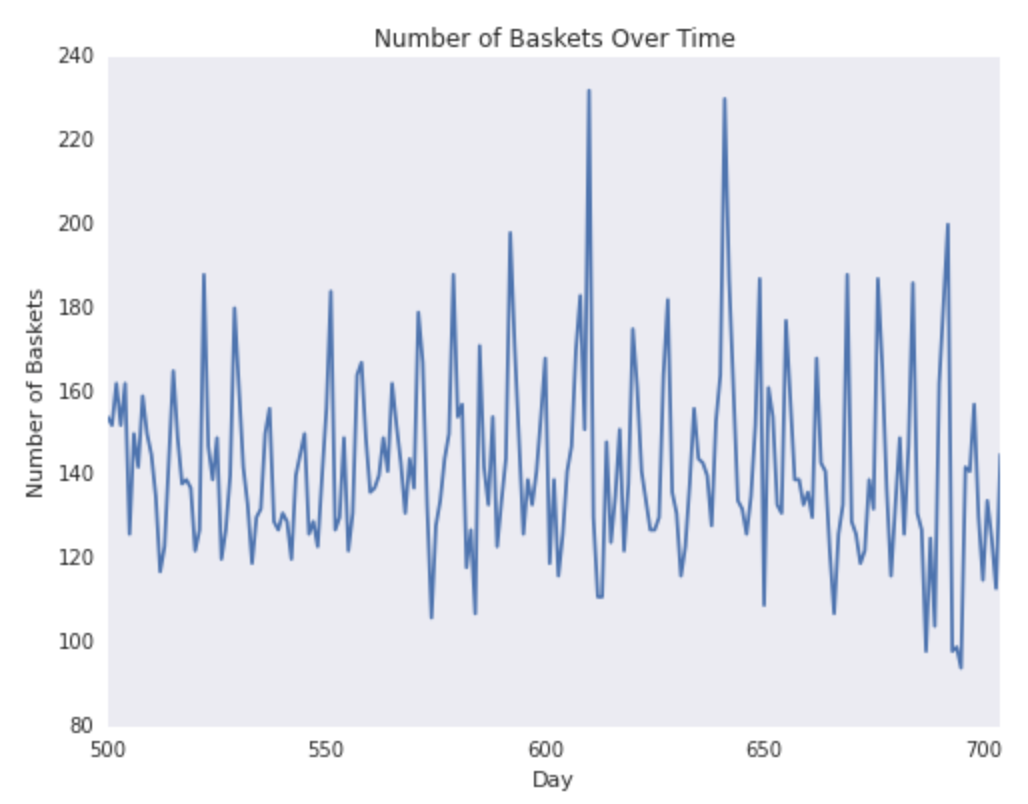
\includegraphics[width=5in]{../slides/figure1.png}
    \caption{Number of Baskets over time.}
\end{figure}

\end{document}
